\documentclass[article, french]{yReport}

\usepackage{lettrine}
\usepackage{multicol}
\setlength{\columnsep}{\marginparsep}

\author{Harvey Sheppard}
\subtitle{Géographie}
\title{Géopolitique\\et Sécurité informatique}

\makeatletter
\let\runauthor\@author
\let\runtitle\@title
\makeatother


\DeclareDocumentCommand{\sideDate}{m}{\vspace{1mm}{\normalsize\lightBoldFont#1\\}}





\begin{document}
	\titleTwo[images/anonymous.png]
	
	\startcontents
	\printMarginPartialToc[1][En Bref]
	
	\section{Introduction}
	\enquote{Internet}...
	Aujourd'hui, avec l'avènement des smartphones, le réseau électronique s'est infiltré partout.
	Son omniprésence semble faire penser à certains qu'Internet est un droit fondamental de l'Homme.
	Qui d'entre-nous ne s'est jamais senti bafoué par une mauvaise connectivité?
	
	L'expansion extrêmement rapide de ce moyen de communication dont les débuts remontent à il y a une cinquantaine d'années%
	\sideNote{\sideTitleColor{Petit historique d'Internet}\\
		\sideDate{1934}Paul Otlet publie une vision prémonitoire de l'avènement d'Internet\\
		\sideDate{1961}Premiers articles sur la communication par paquets\\
		\sideDate{1965}Première communication longue distance entre ordinateurs\\
		\sideDate{1969}ARPANET, le réseau développé par l'armée américaine et ancêtre d'Internet, acquiert 4 n\oe uds\\
		\sideDate{1972}Création du système de message par Internet -- les e-mails -- et première démonstration publique du réseau\\
		\sideDate{1989}Tim Berner Lee au CERN décrit les bases du web (page web, site web, etc.)\\
		\sideDate{1992}Les ordinateurs sont devenus $10^9$ fois plus rapides qu'au début d'ARPANET, la bande passante est 20 millions de fois supérieure et Internet comporte un million d'hôtes\\
		\sideDate{1998}Fondation de Google Inc.\\
		\sideDate{2016}Internet compte 3,2 milliards d'internautes et c'est 205 milliards d'e-mails qui sont envoyés \textit{chaque jour}\\
	}
	pose cependant des questions parmi lesquelles celle de la sécurité.
	Initialement développé par l'armée américaine, ce réseau ne s'est jamais vraiment détaché des infrastructures vitales (armée, production et distribution d'énergie, gouvernements, etc.).
	Et si l'interconnexion d'ordinateurs de par le globe permet de mettre en commun les connaissances et d'augmenter la quantité d'informations échangées, elle expose aussi à tous des machines critiques pour la survie de nations entières.
	
	Internet est un formidable moyen de communication qui a révolutionné notre mode de vie.
	Il a fait avancer la science et permis à l'humanité de se développer à un rythme jusqu'ici inégalé dans l'histoire.
	Mais c'est également un vecteur de fragilité; sa création a exposé au monde beaucoup de systèmes essentiels et les rend ainsi susceptibles d'être la cible d'attaques.
	
	Depuis la création du réseau, de multiples attaques visant des individus ou des États ont été constatées\sideNote{Cet article traitant de géopolitique, nous ne nous intéresserons qu'aux attaques contre des États dans ce document.}.
	Nous nous proposons d'en détailler certaines dans la suite de ce texte, puis de discuter des modifications profondes qu'Internet a amené dans le cadre de la géopolitique.
	
	\section{État contre État}
	L'histoire de l'humanité est entachée de guerres mêlant toutes les ethnies et tous les peuples.
	La taille des armées engagées dans de tels conflits a, au fil de l'histoire, continuellement augmenté pour atteindre, peut-être, son paroxysme lors de la Seconde Guerre Mondiale.
	Mais les guerres ont récemment changé d'apparence.
	Le facteur déterminant n'est plus le nombre de soldats allant se battre, mais la technologie et l'information dont chacun des partis dispose.
	Le conflit moderne, restant tout à fait meurtrier, ne se mène plus la baïonnette à la main mais plutôt le clavier sous les doigts et l'écran devant les yeux.	Peu étonnant dès lors, qu'Internet devienne un facteur clé de la guerre du 21\textsuperscript{e} siècle.
	
	Un premier exemple d'un tel changement est celui du virus\sideNote{Voir l'annexe \ref{app:typeVirus}} Stuxnet; découvert en 2010 et probablement développé par les États-Unis et Israël.
	Il visait spécifiquement les ordinateurs des centrales nucléaires iraniennes et corrompait les programmes contrôlant les centrifugeuses d'enrichissement d'uranium, le tout résultant en de mystérieuses et inexplicables pannes.
	Le but d'une telle entreprise étant ici de ralentir le programme nucléaire iranien en empêchant la trop grande création d'uranium militaire.
	L'incidence d'un tel cas sur la géopolitique semble évidente: une guerre larvée, dématérialisée, se déroule maintenant sur Internet entre les États pour des questions d'ordre politique.
	
	\begin{figure}[ht!]
		\sideCaptionOf{figure}{Fonctionnement du virus Stuxnet}%
		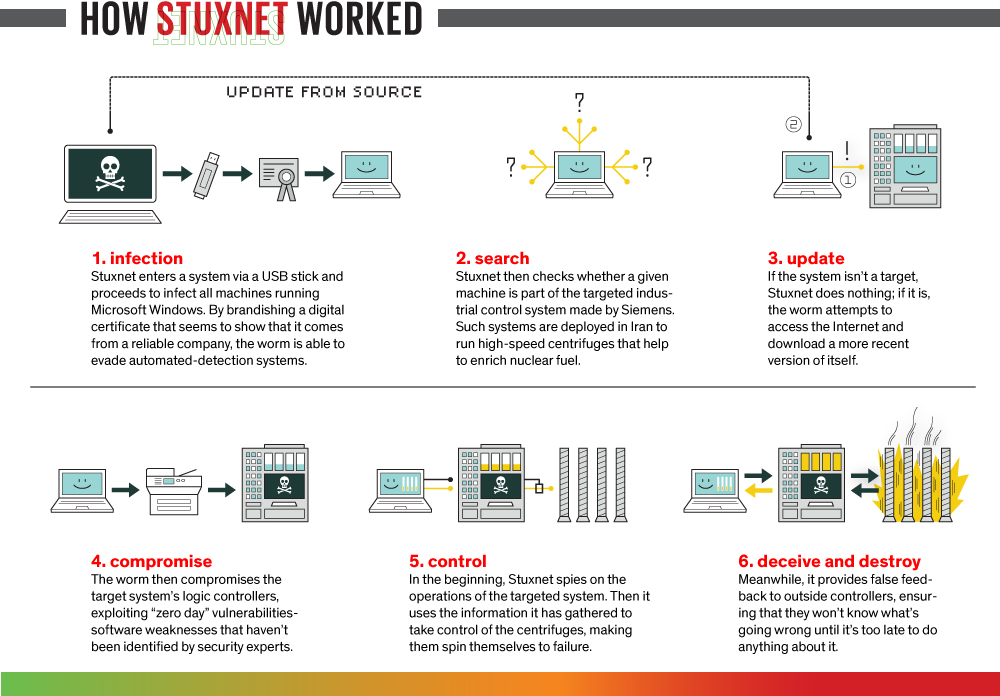
\includegraphics[width=\textwidth]{images/stuxnet.jpg}
		\label{fig:stuxnet}
	\end{figure}
	
	Autre coin du monde, autre conflit...
	Nous voilà maintenant dans l'ouest de l'Europe, à la frontière entre la Russie et l'Ukraine.
	Les tensions entre les deux nations induites par les conflits d'intérêts autour de la Crimée inquiètent.
	Et soudain, au soir du 23 décembre 2015, la région d'Ivano-Frankivsk sombre dans le noir total.
	La panne d'électricité touche près de 700'000 foyers durant plusieurs heures.
	
	Pourquoi vous parler de \textit{cette} panne? Parce que la défaillance des services serait due à une attaque informatique lancée par des hackers pro-russe qui auraient utilisé une version modifiée du virus BlackEnergy\sideNote{Le crimeware (logiciel destiné à l'automatisation de tâches criminelles) BlackEnergy rassemble un certain nombre d'outils informatiques permettant de multiples actions néfastes: spam, création de réseaux de botnets, pénétration de toutes sortes de dispositifs (routers, ordinateurs, contrôleurs de machines industrielles, etc).
	Il est principalement utilisé par les réseaux de hackers russes et a déjà servi à attaquer de grandes organisations comme l'OTAN.} et que Kiev n'a pas manqué de pointer du doigt Moscou.
	
	De fait, cette attaque marque un tournant dans l'histoire du hack.
	C'est la concrétisation d'un scénario catastrophe jusqu'ici resté hypothétique: les systèmes essentiels d'un pays sont touchés.
	La situation n'a causé aucun mort ni eu de conséquences trop sérieuses mais qu'en aurait-il été si les pirates avaient pris le contrôle des services de distribution d'eau, détruit le système de production/distribution d'énergie ou encore mis hors-service les réseaux de transport et de communication?
	
	
	\section{Individu contre État}
	Le conflit se déplace vers des éthers composés de zéros et de uns.
	Et il est évident que les États, disposant de moyens conséquents, peuvent développer des armes digitales puissantes.
	Cependant, Internet est un univers dont les règles ne correspondent en rien au monde matériel.
	Pour dupliquer un char d'assaut, il faut de l'argent, des hommes, des matières premières, beaucoup de connaissances scientifiques, etc.
	Pour dupliquer un virus, deux clics suffisent.
	Et ce changement de paradigme a opéré une véritable révolution.
	De nos jours, la participation au conflit digital n'est plus réservée aux seuls États mais est accessible à chaque individu (que cela soit de manière volontaire ou non\sideNote{Des milliers d'ordinateurs particuliers de par le monde sont contaminés par des virus les utilisant, par exemple, comme des relais pour des attaques par déni de service (voir section \ref{app:DoS}).}).
	
	Les dénonciations formulées par Edouard Snowden\marginElement{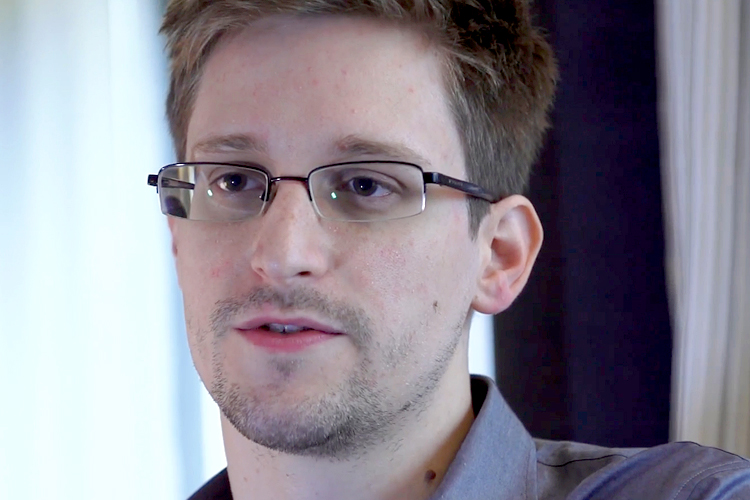
\includegraphics[width=\linewidth]{images/edwardSnowden.jpg}}\sideNote{\sideTitleColor{Edward Snowden}\\Edward Snowden (né le 21 juin 1983), ancien agent de la CIA et de la NSA, est mondialement connu pour avoir copié des centaines de milliers de documents secrets de services comme la NSA, l'AIC (Australian Intelligence Community) ou encore le GCHQ (Government Communications Headquarters) et les avoir, par idéologie, rendus publics.
	Il est actuellement poursuivi par les États-Unis pour violation de l'\textit{Espionage Act} de 1917 et vol de propriétés du gouvernement américain.
	Présentement en exil en Russie, il cherche asile quelque part dans le monde et risque des dizaines d'années de prison s'il est arrêté.} sont un bon exemple de cette participation particulière.
	Dans ce cas, un seul individu a dévoilé les méfaits digitaux perpétrés par trois États\marginElement{Documents publiés par Edward Snowden:\\\url{https://search.edwardsnowden.com}}\sideQuote[Edward Snowden]{Je ne peux, en bonne conscience, permettre au Gouvernement des États-Unis de détruire l'intimité, la liberté d'Internet et les privilèges élémentaires autour du monde, avec cette machine de surveillance massive qu'ils construisent secrètement.} --- les États-Unis, l'Angleterre et le Canada.
	Ces derniers surveillaient et surveillent encore, à n'en pas douter, les communications passant par Internet.
	Le programme PRISM,\marginElement{
\includegraphics[width=\linewidth]{images/PRISM.png}} un des logiciels développés dans le cadre de cette coopération, est chargé de collecter des données de toutes les grandes entreprises du net comme Google, Microsoft, Yahoo, Facebook ou Youtube et permet aux agents l'employant d'obtenir toutes sortes d'informations normalement privées (chat, commentaires, photos, e-mails, téléphonie par Internet, etc).
	L'annonce publique d'une telle surveillance le 5 juin 2013 avait eu un retentissement énorme dans les médias et pose la question des droits fondamentaux de l'individu face à l'État et celle de la vie privée.
	
	Un autre cas où Internet joue un rôle prépondérant pour la géopolitique: le Djihad.
	Avec le printemps arabe le Moyen-Orient est devenu le théâtre de la montée en force de groupes islamistes radicaux.
	Et ces derniers font maintenant du recrutement en ligne par les réseaux sociaux, atteignant ainsi des populations plus éloignées que celles résidant au Moyen-Orient; c'est l'Europe et plus généralement les pays développés comprenant des minorités musulmanes qui sont concernés\sideNumber{240}{C'est le nombre de français qui seraient partis faire le Djihad en Syrie.
	Ce sont, en moyenne, des jeunes entre 18 et 25 ans qui partent, contactés directement par des vétérans djihadistes.}.
	Le groupe État islamique ne s'arrête pas seulement au recrutement, le défacement de site web est également devenu un outil.
	L'attentat de Charlie Hebdo fut d'ailleurs accompagné de centaines de sites web français piratés\sideNote{Quelques exemples de sites web défacés:\begin{sideItems}
		\item Site du Mémorial de Caen
		\item Site du Palais des Papes
		\item Site de la cathédrale de Nantes
	\end{sideItems}}.
	Internet est un instrument de propagande, mais aussi, et peut-être plus encore, de communication pour ces groupes.
	Il leur permet d'échanger informations et renseignements anonymement.
	Pour cette raison, les États-Unis ont lancé une véritable guerre informatique contre l'EIIL.
	6000 soldats de l'US Army, spécialisés dans divers domaines digitaux, ont été placés sous la direction de l'amiral Michael Rogers (directeur de la NSA) avec pour but de surcharger les réseaux du groupe extrémiste, qui, ainsi, perdrait sa capacité à commander ses forces et son économie.
	
	D'autres exemples de particuliers jouant un rôle important sur Internet viennent rapidement à l'esprit; pour n'en citer qu'un: Anonymous.
	On assiste ici à un véritable changement d'échelle.
	L'individu a maintenant son mot à dire dans notre univers globalisé, il peut être entendu et ne saurait être ignoré des plus grands.
	
	\section{Conclusion}
	Soulignons-le encore, la création du réseau Internet est à marquer d'une pierre (blanche ou noire, chacun décidera) dans l'histoire de l'humanité.
	Ce nouveau moyen de communication a supprimé la notion de frontière en ligne et conduit à un bouleversement profond de notre mode et qualité de vie.
	Les conflits changent, les règles changent, les facteurs déterminants changent.
	
	Toutes ces modifications apportent beaucoup de questions, auxquelles les lois peinent à répondre, car elles n'ont pas encore eu le temps de s'adapter (ce qui mène parfois à des procès partiaux\sideNote{Ross Ulbricht, fondateur du site web \textit{The Silk Road} (site de vente de drogue sur le dark net, visant à démocratiser la vente et l'achat de drogue pour diminuer la criminalité associée à ce commerce), s'est vu condamné à perpétuité par la juge fédérale Katherine Forrest (États-Unis), alors que les preuves de l'accusation montraient de multiples incohérences et que certaines de ces preuves avaient probablement été obtenues illégalement.}).
	Internet est un lieu d'immense liberté, peu régulé.
	Il est facile d'y entrer dans l'illégalité et difficile de punir les coupables.
	
	C'est un outil dont se servent les terroristes et les criminels pour faire du recrutement, de la vente et de l'achat d'armes et de drogues; il est aussi un des derniers moyens de communication dont disposent les opprimés, il est une façon d'obtenir un peu d'anonymat, il est aussi la porte ouverte à la surveillance de masse.
	Ses multiples facettes sont innombrables.
	
	Faut-il faire primer les États sur les individus? Les États peuvent-ils se permettre de dépasser le cadre légal en ligne (surveillance, attaque d'autres États)? La diffusion de logiciels de cryptographie puissants à tout un chacun est-elle à cautionner?
	
	Ces questions font couler beaucoup d'encre.
	Et il semble difficile de leur trouver une bonne solution.
	Mais une chose est sûre: l'informatique a une incidence importante sur la géopolitique.
	Elle va même très certainement augmenter.
	Ce qui est initialement une science va maintenant prendre une place de plus en plus grande dans la création, le déroulement et la résolution des conflits nationaux et internationaux.
	N'oublions donc jamais que...
	
	\blockQuote{Science sans conscience n'est que ruine de l'âme.}
	
	
	
	\vfill
	\drawBackground\startBackground
	\begin{whole}
		{\color{mainColor}\huge\fontspec{Fira Sans Book} Quelques chiffres d'internet}
		\begin{multicols}{2}
		\vspace*{0mm}\bigNumber{205 mia}\\[1mm]
		C'est le nombre d'emails envoyés \textit{chaque jour} de part le monde.
		En tout, cela fait 74 trillions par année.
		
		\vspace*{3mm}\bigNumber{1\$ mia}\\[1mm]
		C'est l'argent qu'un groupe de hacker d'Europe de l'Est nommé Carbanak a réussi à voler en deux ans grâce à des attaques de social engineering visant des centaines de banques.
		
		\vspace*{3mm}\bigNumber{38,5\$ mia}\\[1mm]
		C'est le coût en dollar des dommages qu'aurait causé MyDoom dans les années 2004.
		Utilisant les pièces jointes des emails pour se propager, ce vers est connu pour être celui qui s'est disséminé le plus rapidement dans l'histoire de l'informatique.
		
		\columnbreak
		\vspace*{0mm}\bigNumber{1,6 mia}\\[1mm]
		C'est le nombre d'utilisateurs Facebook en 2016.
		
		\vspace*{3mm}\bigNumber{10 mio}\\[1mm]
		C'est le nombre d'attaques que subissait le département de la sécurité du gouvernement américain en 2012 \textit{par jour}.
		
		\vspace*{3mm}\bigNumber{527 mio}\\[1mm]
		C'est la quantité de tonnes de $\mathrm{CO_2}$ émise par la production de l'énergie nécessaire à Internet.
		C'est équivalent à la pollution générée par la flotte aérienne mondiale.
		De fait, chaque recherche sur Google génère 0,2 gramme de $\mathrm{CO_2}$ (un millier de recherches génère la même pollution qu'une voiture qui roule sur un kilomètre).
		\end{multicols}
	\end{whole}
	\stopBackgroundPageBottom
	
	
	\appendices
	\renewcommand{\thesection}{\Alph{section}}
	\section[Types d'attaques informatiques]{Attaques digitales et\\programmes malveillants}
	\label{app:typeVirus}
	La sécurité informatique est un domaine extrêmement complexe et vaste.
	Il est par conséquent absolument impossible de dresser une liste complète de toutes les attaques possibles.
	En voici cependant une brève liste.
	
	Les attaques digitales n'ont pas forcément ni le même but ni la même cible.
	On parlera d'attaques passives dans le cas où elles se contentent de récolter des informations.
	À l'inverse, l'attaque active tente de pénétrer un réseau, d'accéder à des ordinateurs puis de les pirater, d'obtenir plus de privilèges sur les machines compromises\sideNote{Cette aspect du hack se nomme l'escalade de privilège et a pour but d'obtenir les droits administrateurs voire système (ce que normalement aucun utilisateur ne peut faire) sur un ordinateur.}, etc.
	Plus qu'écouter, elle agit.
	
	Pour ce qui est des cibles, elles peuvent être de types très différents: réseaux, ordinateurs personnels, smartphones, routers, voitures connectées, compte email, site web, etc.
	De même, les buts recherchés peuvent varier immensément: défigurer un site web pour des raisons idéologiques, le mettre simplement hors-ligne, dériver les communications sortant d'une entreprise afin de pouvoir les écouter, usurper l'identité de quelqu'un en passant par son profil Facebook, gagner de l'argent en craquant des codes de cartes bancaires, etc.
	Internet est véritablement une jungle ou le plus intelligent dicte sa loi.
	
	\sideFigure{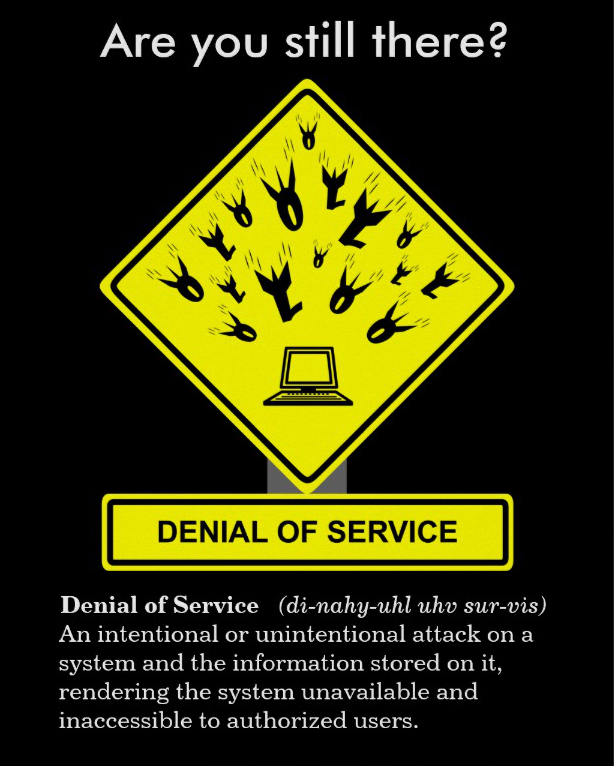
\includegraphics[width=\linewidth]{images/DoS.jpg}}
	\subsection{Déni de service (distribué)}
	\label{app:DoS}
	L'attaque par déni de service (distribué) nommée DoS (Denial of Service) ou DDos (Distributed Denial of Service) est une des attaques les plus courantes quand la cible est un site web.
	Elle consiste à demander des centaines de milliers de fois à un serveur web d'afficher une page du site qu'il héberge.
	La machine va tenter de faire cela au mieux et soutiendra, un moment du moins, la demande.
	Mais à terme la quantité de demandes trop importante fera surchauffer le serveur qui cessera de servir la page: le site web est alors mis hors-ligne.
	De telle attaques nécessitent d'être maintenues pour perdurer dans le temps.
	L'attaque distribuée implique non pas un seul attaquant mais des centaines voire des milliers de machines (souvent des réseaux de botnets).
	Elles sont beaucoup plus efficaces et difficiles à contrer.
	
	\sideFigure{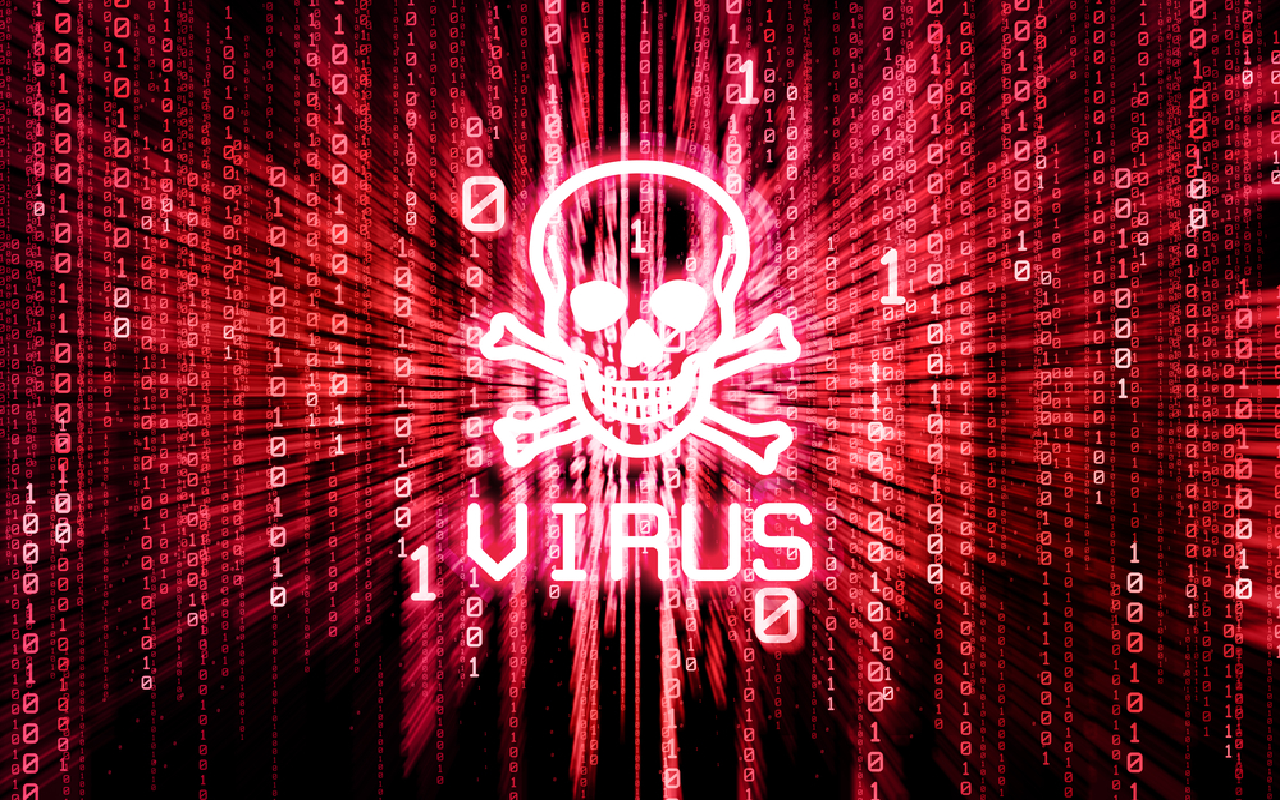
\includegraphics[width=\linewidth]{images/virus.png}}
	\subsection{Virus, vers et chevaux de Troie}
	Sans rentrer dans trop de détails, ces trois catégories de programmes infectent les ordinateurs.
	Ils ont la capacité de se répliquer, soit à d'autres endroits sur une même machine, soit via le réseau, sur d'autres ordinateurs et donnent à l'attaquant de multiples possibilités: vol d'informations, accès secret à la machine, escalade de privilèges, transformer l'ordinateur en \enquote{zombie} (il fera alors partie d'un réseau de botnet), etc.
	Pour compromettre la machine, ils utilisent des exploits (voir section \ref{sec:exploits}).
	
	\newpage
	\sideFigure{\vspace*{2mm}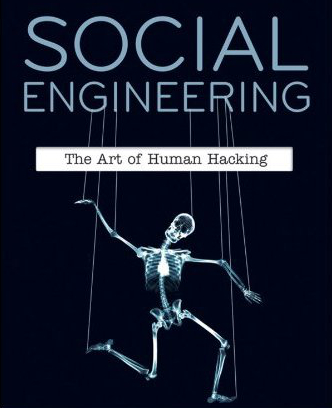
\includegraphics[width=\linewidth]{images/socialEngineering.jpg}}
	\subsection{Social Engineering}
	Peut-être l'attaque la plus dangereuse, elle vise le maillon le plus faible dans la chaine de défense d'un système informatique: le facteur humain! Elle consiste à manipuler des membres d'une entreprise ou d'un État par téléphone, via des emails ou tout autre moyen pour les pousser à donner mots-de-passe, adresses e-mail, adresses IP, etc.
	C'est très probablement aussi l'attaque dont on se méfie le moins car elle est moins connue et les entreprises, si elles investissent volontiers dans des anti-virus, ne pensent que trop rarement à former leurs membres.
	
	\subsection{Pièces jointes corrompues}
	À l'inverse, cette attaque figure parmi les plus connues, elle consiste à envoyer une pièce jointe par e-mail contenant un fichier modifié de façon à pouvoir exploiter une faille dans le programme qui le lira (une faille dans le programme Word par exemple) pour pouvoir exécuter du code arbitraire sur la machine cible.
	
	\sideFigure{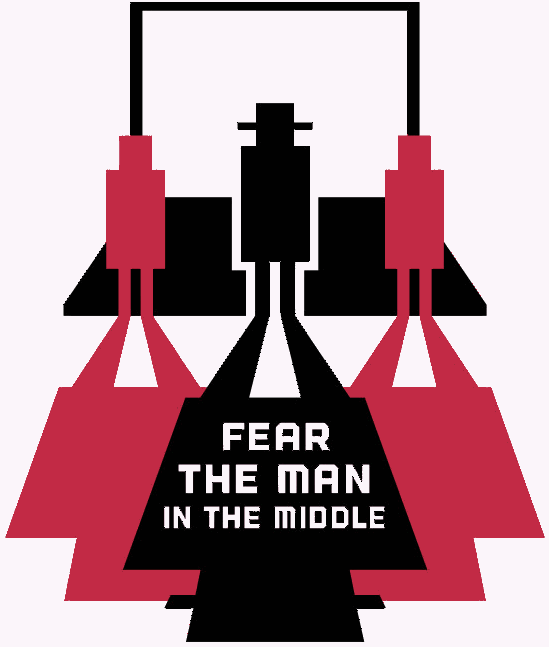
\includegraphics[width=\marginparwidth]{images/manInTheMiddle.png}}
	\subsection{Man in the middle}
	Dans cette attaque, l'attaquant dévie les communications entre deux personnes afin qu'elles passent par lui.
	Il peut ainsi \enquote{écouter} tout ce qui passe par le réseau entre ces deux individus.
	Il est même possible de modifier les données au vol afin que le contenu échangé corresponde à ce que l'attaquant veut qu'il soit.
	Certains protocoles de sécurité permettent d'éviter ce genre d'attaque mais elle reste très facile à exécuter sur certains dispositifs comme les Wifis.
	
	\sideFigure{
\includegraphics[width=\marginparwidth]{images/xss.jpg}}
	\subsection{Faille XSS (Cross Site Scripting)}
	Aussi connue sous le nom d'injection SQL, cette attaque se décline en deux versions.
	Dans la première, nommée réfléchie (comme dans réfléchissant) ou non-persistante, des adresses web frauduleuses ou des formulaires remplis de façon particulière conduisent à l'exécution de code indésirable du côté client (par opposition au côté serveur).
	C'est la plus bénigne des deux dans le sens qu'elle ne change rien sur le serveur du site web et qu'elle ne peut causer que des dégâts limités chez le visiteur, car les langages clients sont généralement limités (vol de mots-de-passes, modification du contenu du site web du côté client uniquement).
	La deuxième, beaucoup plus dommageable, consiste à rentrer du code (SQL généralement) dans des formulaires mal protégés de sites web afin d'afficher ou de modifier des informations de la base de données normalement inaccessibles aux visiteurs.
	Cette dernière modifie le site web.
	
	\subsection{Exploits et Zero-days}
	\label{sec:exploits}
	La plupart des attaques (pièce jointe malicieuse, virus, etc.) utilisent des exploits pour infecter les ordinateurs.
	Un exploit est une faille dans du code qui permet de détourner l'utilisation première à laquelle il était destiné.
	Elles peuvent être de types très variés.
	Les failles XSS, décrites plus haut, en sont un exemple.
	Elles fonctionnent car l'utilisateur peut entrer du code dans un champ texte (le programmeur ne vérifie pas suffisamment que l'entrée de l'utilisateur est celle attendue).
	Mais il en existe beaucoup d'autres.
	Une parmi les plus connues se nomme Buffer Overflow.
	Elle consiste à rentrer une chaine de caractères beaucoup plus longue que celle attendue par l'ordinateur.
	L'attaquant dépasse la zone mémoire allouée pour la chaine de caractères et écrit alors dans la mémoire temporaire de l'ordinateur (la RAM).
	Il peut ainsi lui faire exécuter du code arbitraire.
	Cette attaque figure parmi les plus répandues\sideNote{Le Buffer Overflow est une faille très répandues, car les langages C et C++, énormément utilisés depuis les années 80, ne vérifient pas que le contenu écrit dans la mémoire RAM ne dépasse pas la taille limite allouée.} et les plus dangereuses.
	Bien menée, elle peut conduire à la corruption totale d'un ordinateur (obtention des privilèges administrateur voire système).
	
	La plupart des exploits, une fois découverts, sont publiés et les responsables du code écrivent un correctif sous la forme d'une mise à jour.
	Cependant, les personnes qui cherchent ces exploits gardent parfois pour elles leurs découvertes, qui restent non-corrigées.
	C'est alors un exploit zero-day, une faille jusque-là inconnue du public dont il est quasiment impossible de se protéger.
	De telles faiblesses sont monnayées au prix fort sur le dark-net et parmi les acheteurs figurent parfois des gouvernements dont l'intention n'est pas de rendre leur achat public.
	
	\newpage
	\section{Red October}
	\begin{figure}[ht!]
		\vspace*{3mm}
		\begin{centered}
			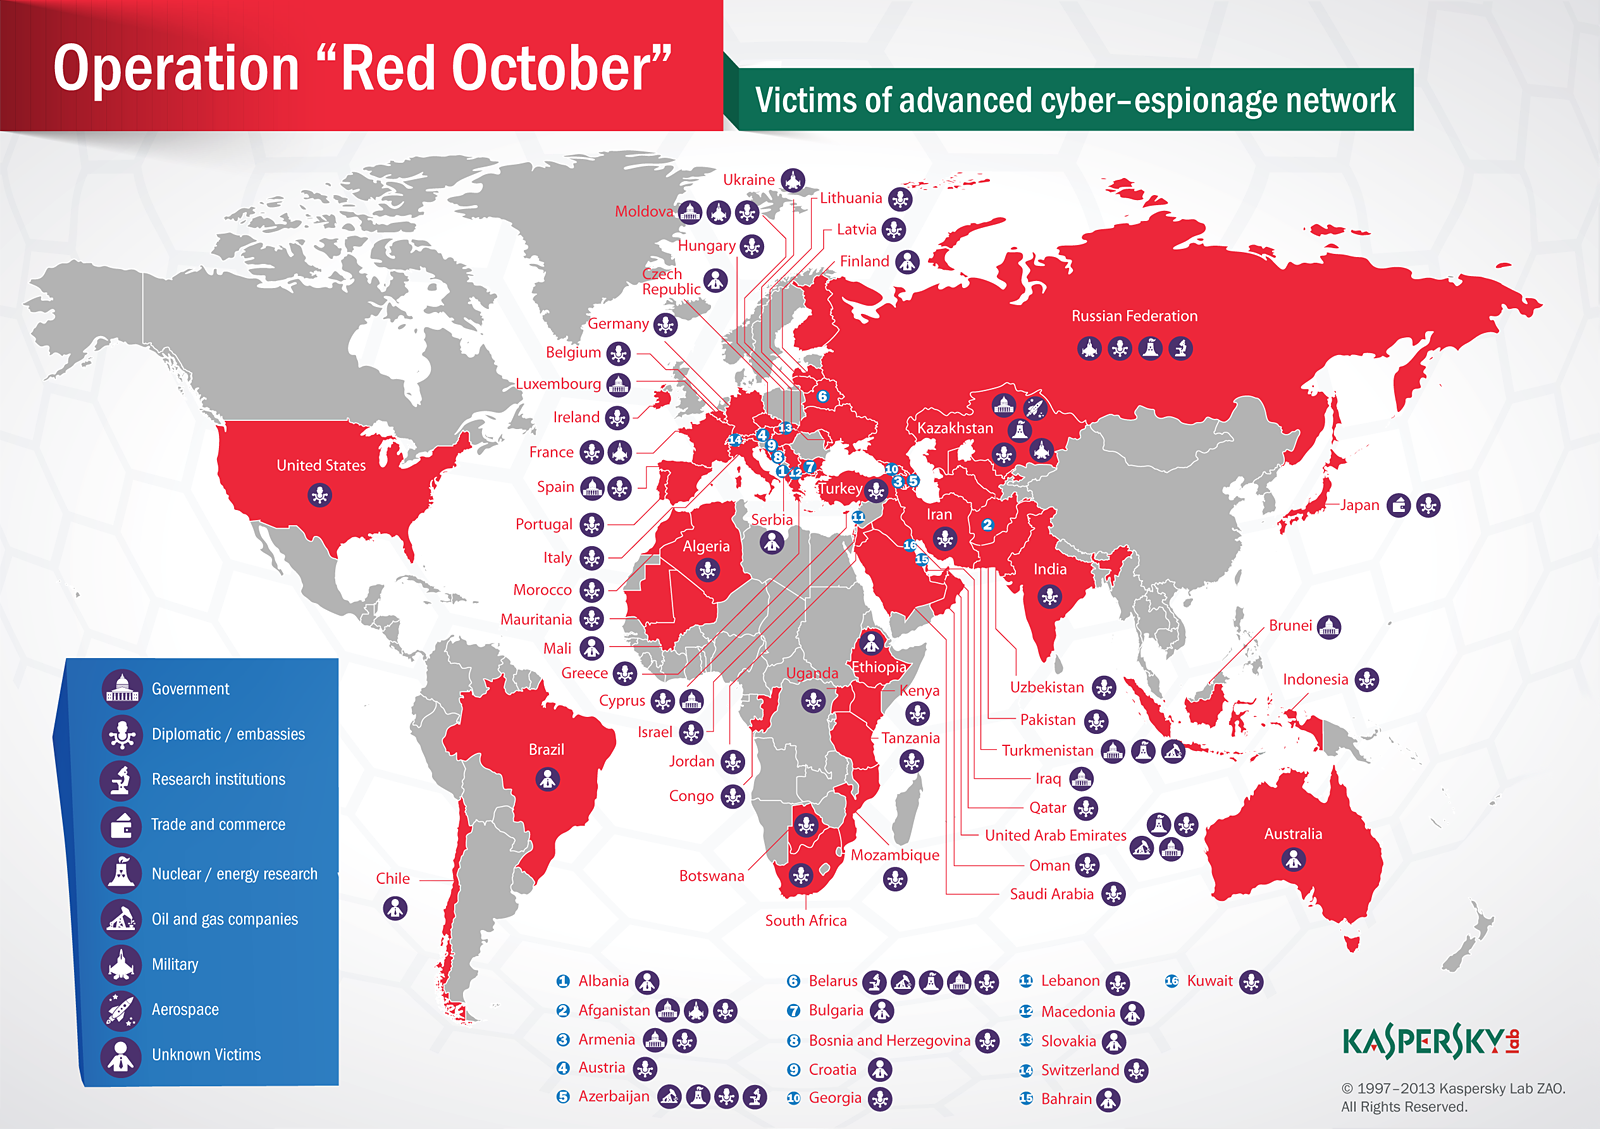
\includegraphics[width=\linewidth]{images/redOctober.png}
		\end{centered}
		\vspace*{5mm}
	\end{figure}
	
	L'opération \enquote{Red October} était une campagne de piratage lancée depuis au moins 5 ans avant d'être découverte, en janvier 2013, par le laboratoire de recherche Kaspersky.
	Cette attaque d'envergure visait principalement les ambassades et les gouvernements.
	Elle ne se limitait cependant pas à ces derniers: instituts de recherche scientifique, centrales nucléaires, bourses et services de l'aviation furent aussi touchés.
	En tout, c'est plus de 60 nations qui sont concernées, principalement dans l'Europe de l'Est et l'Asie, mais aussi certains pays \enquote{du nord} comme la Suisse ou les États-Unis.
	\marginElement{Petite anecdote intéressante, l'opération \enquote{Octobre Rouge} tire son nom de la nouvelle \enquote{The Hunt for Red October} par Tom Clancy.
	Red October est le nom d'un sous-marin russe dans la nouvelle.\\[\baselineskip]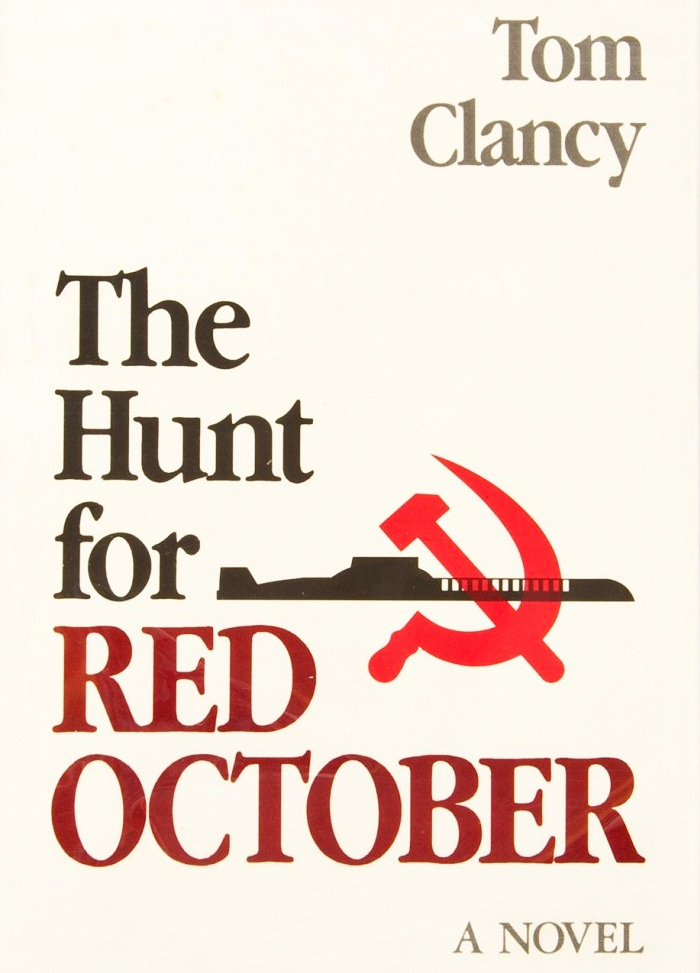
\includegraphics[width=\linewidth]{images/theHuntForRedOctober.jpg}}
	
	Les victimes étaient infectées via une pièce jointe corrompue: un document Word ou Excel malicieux.
	Le virus ajouté à l'ordinateur relevait lui par contre d'une grande complexité.
	Propre au groupe pour l'instant inconnu de hackers menant cette opération, le programme Rocra  (condensation de \enquote{Octobre Rouge} en russe) pouvait être augmenté de modules de cryptographie avancée, de modules pour les téléphones mobiles et même de code pour pouvoir réinfecter les machines qui auraient supprimé le virus principal.
	
	Utilisant près de 60 serveurs de relai, Octobre Rouge a infecté des centaines d'ordinateurs clés (gouvernements, institutions diplomatiques, OTAN, etc.) de par le monde.
	L'attaque n'a pu être reliée à aucun pays particulier mais l'exploit utilisé fut développé par des hackers chinois et le programme Rocra est écrit par des personnes russophones.
	
	On estime que 7 terabytes\sideNote{1 terabyte = 1000 gigabytes} de données furent volés.
	Les types de fichiers concernés étaient divers: pdf, fichiers Excel, fichiers Word, etc.
	Cependant, beaucoup de fichiers portant l'extension .acid furent dérobés.
	Ces derniers étaient générés par le programme Acid Cryptofiler, un logiciel de cryptographie employé par l'armée française et l'OTAN.
	
	L'influence d'une telle violation n'est pas à minimiser.
	Qui sait quels secrets furent volés ou déchiffrés.
	L'impact sur la géopolitique est ici plus évident encore que dans les exemples précédant, car l'attaque se concentrait sur la collecte d'informations touchant à ce domaine.
	Personne ne sait à quelles fins ces dernières furent utilisées.
	Elles ont probablement été vendues sur le dark-net ou utilisées directement.
	
	\vfill
	\hfill\authorBlock{
			\authorName{Harvey Sheppard}
			\blockLine{\extraVerticalSpace{\FA\symbol{"F19D}}}{My School}
			\blockLine{}{The Class}
			\authorAdressLineOne{my street, 6}
			\authorAdressLineTwo{my city, Canada}
			\authorPhone{my phone number}
			\authorMail{my email@test.com}
		}
	
\end{document}